\documentclass[a4wide,12pt]{report}
\usepackage[utf8]{inputenc}
\usepackage[IL2]{fontenc}
\usepackage{listings}
\usepackage{amssymb}
\usepackage{amsmath}
\usepackage{mathtools}
\usepackage{url}
\usepackage{graphicx}
\usepackage[czech]{babel}
%\usepackage{fullpage}
\usepackage[top=22mm, bottom=30mm, left=35mm, right=25mm]{geometry}
\usepackage{tikz}
\usepackage{subfig}
\usepackage{float}
\usepackage{algorithm}
\usepackage{algorithmic}
\usepackage[all]{xy}
\usetikzlibrary{shapes.misc}
\newcommand{\HRule}{\rule{\linewidth}{0.5mm}}
\hyphenation{NetLogo}
\title{sds}
\author{Marek Bryša}
\date{Brno 2011}
\begin{document}
\thispagestyle{empty}
\pagebreak
\mbox{}% to get into horizontal mode
\vfill

\begin{center}
% Upper part of the page

\includegraphics[width=0.2\textwidth]{./znak_MU_cerny.eps}\hspace{2cm}

\includegraphics[width=0.2\textwidth]{./znak_PrF_cerny.eps}\\[1cm]    

{\LARGE Masarykova univerzita}\\[0.5cm]
{\LARGE Přírodovědecká fakulta}\\[0.5cm]
{\LARGE BAKALÁŘSKÁ PRÁCE}\\[0.5cm]
{\LARGE Marek Bryša}\\[0.5cm]

{ \huge \bfseries Lager brewing techniques}\\[0.4cm]
{\large Vedoucí práce: Ing. Michal Kvasnička, Ph.D.}\\[0.5cm]
{\large Studijní program: Aplikovaná matematika}\\
{\large Studijní obor: Matematika-Ekonomie}\\[0.5cm]
{\large 2011}\\
\vspace{5cm}

\vfill
\pagebreak
% end of page 

\end{center}

\newpage
\thispagestyle{empty}
pisemne zadani
\newpage
\thispagestyle{empty}
\vspace{2cm}
\noindent
Děkuji panu Ing. Michalu Kvasničkovi, Ph.D. za rady a připomínky cenné nejen při tvorbě této práce.\\
Děkuji paní Kateřině Kšicové za poskytnutí informací o fungování prodejní sítě Oriflame.
\vfill
\noindent
Prohlašuji, že jsem svou bakalářskou práci napsal samostatně a výhradně s použitím citovaných pramenů.\\[3cm]
V Brně, dne \today \hfill Marek Bryša\hspace{3cm}
\vspace{1.5cm}
\newpage
\newpage
\thispagestyle{empty}
abstrakt
\newpage
\tableofcontents

\chapter*{Úvod}
\addcontentsline{toc}{chapter}{Úvod}
Tato bakalářská práce se bude zajímat o studium síťového marketingu z ekonomického pohledu. To je systém, kde se samotní spotřebitelé mohou stát za učitých podmínek prodejci. K tomu a zejména k přivedení dalších lidí se je provozovatel snaží finančně motivovat. Tím provozovatel ušetří náklady na budování kamenných prodejen. Cílem bude analýza vzniku sítě, průběhu jejího šíření a její výsledné struktury. Pokusíme se také nalézt příjmové a nákladové funkce provozovatele i jednotlivých členů a z nich pro ně odvodit doporučení vedoucí k optimalizaci zisku.

Metodou zvolenou k dosažení těchto cílů je vytvoření počítačového modelu se snahou o co nejvěrnější napodobení skutečnosti. Na něm pak budeme provádět simulace a experimenty a jejich výsledky interpretujeme pomocí statistických a ekonometrických nástrojů. Z důvodu reálné využitelnosti získaných závěrů bude tato práce konkrétně modelovat systémem síťového marketingu, který používá firma Oriflame\footnote{Oriflame --- Přírodní švédská kosmetika, \url{http://cz.oriflame.com/index.jhtml}}. Ten byl zvolen pro svou relativní jednoduchost, úzké zaměření na kosmetické výrobky, což usnadní ekonomické úvahy, a autorovu blízkost k současným členům sítě. Informace přensném fungování systému byly získány z interních materiálů firmy a osobních rozhovorů se zaměstnanci a členy prodejní sítě.

První kapitola poskytne úvod do fungování sítě firmy Oriflame. Seznámíme se s konkrétními parametry, na kterých je postavena, a s motivací, kterou firma svým prodejcům poskytuje. Ve druhé kapitole se budeme zabývat tvorbou sociálních vazeb, ekonomickými úvahami o síti a implementací obojího do počítačového modelu. Třetí kapitova bude věnována samotné analýze chování sítě a jejích členů, provádění multiagentových simulací a interpretaci získaných dat.
\chapter{Prodejní síť Oriflame}
Tato kapitola nabízí úvod do fungování prodejní sítě Oriflame a jejích parametrů. Poslouží jako základ k vybudování počítačového modelu v příští kapitole. Zde se ze začátku seznámíme s historií Oriflame a sortimentem produktů. Dále se budeme věnovat struktuře katalogu, tvorbě cen a podrobně podmínkám, na základě kterých mohou si lidé s Oriflame přivydělat. Závěrem je uveden obrázek s příkladem, jehož účelem je objasnění na první pohled komplikovaného systému.
\section{Historie firmy Oriflame}
Firma Oriflame byla založena v roce 1967 ve Švédsku bratry Jonasem a Robertem Jochnick. Cílem bylo nabídnout lidem přirozenou a přírodní péči o svou pleť. Místo aby nákladně budovali kamenné obchody, rozhodli se dostat prodej přímo do domovů a využít tak vrozenou podnikavost lidí. Tento základní koncept zůstáva po více než čtyřicet let nezměněn. V roce 1990, po po pádu železné opony, firma expandovala po střední a východní Evropě a založila pobočku i v České republice. V roce 2001 dosasáhl počet prodejců zapojených v síti Oriflame na celém světě jednoho miliónu a obrat téměř 450 miliónů EUR.

Sortiment je opravdu široký, katalog obsahuje přes 1 500 výrobků v cenách přibližně od 50 do 1 000 Kč. Většina typů produktů obsahuje několik cenou a kvalitou odlišených řad. Celkově lze říci, že zákazník má možnost nákupu komplexní péče s téměř libovolným rozpočtovým omezením.
\section{Podmínky síťového prodeje}
V této části popíšeme fungování sítě Oriflame na českém trhu. V jiných zemích se mohou zejména parametry mírně lišit.

Každému výrobku jsou v ceníku přiděleny čtyři hodnoty:
\begin{description}
\item[PC] Doporučená prodejní cena spotřebitelům, která je uvedena v katalogu.
\item[NC] Nákupní cena včetně DPH. Za tu prodejci mohou zboží zakoupit v centrech Oriflame a na internetu. V České republice se nyní nachází tři hlavní centra (Praha, Brno, Ostrava) a tři centra (České Budějovice, Olomouc, Plzeň).
\item[OO] Obchodní obrat. Typicky je roven nákupní ceně bez DPH. V případě produktů, které nemají daný objem (např. kartáč na vlasy, houba na mytí), je ještě přibližně poloviční.
\item[BO] Bodové ohodnocení. Na inflaci nezávislý počet bodů, které prodejce nákupem zboží získá. Jestliže cena výrobku důsledkem inflace stoupne, bodové ohodnocení zůstává, a tím se poměr mezi nimi v čase mění. V současnoti jeden bod obdrží za přibližně 13,80 Kč obchodního obratu.
\end{description}
Výjimku tvoří např. tiskoviny, vzorky a oblečení s logem Oriflame, které mají pouze nákupní cenu,  nejsou určeny k dalšímu prodeji a slouží jen jako pomůcka pro prodejce.

Rok firma rovnoměrně rozdělila na 17 období, které odpovídají vydáním katalogů výrobků. Prodejce, který podal v předchozích třech obdobích alespoň jednu objednávku, obdrží sadu tiskovin zdarma, jinak je pro něj téměř nutnost si tištěný katalog zakoupit za TODO:cena katalogu.

Prodejce dále získá body všech lidí které přivedl, těch pod nimi atd. Na konci každého katalogového období dochází k vyhodnocení. Sečtou se všechny body a podle tabulky \ref{tab:perc_level} se určí procentní úroveň.
\begin{table}[htb]
\begin{center}
\begin{tabular}{|l|c|c|c|c|c|c|c|}
\hline
body & $\geq$200 & $\geq$600 & $\geq$1200 & $\geq$2400 & $\geq$4000 & $\geq$6600& $\geq$10000\\\hline
úroveň & 3\% & 6\% & 9\% & 12\% & 15\% & 18\% & 21\%\\\hline
\end{tabular}
\end{center}
\caption{Určení procentní úrovně}
\label{tab:perc_level}
\end{table}
Toto se provede i pro všechny podskupiny. Prodejce pak získá za každou podskupinu:
\begin{equation} \label{eq:spons}
\text{obchodní obrat skupiny} \cdot (\text{procentní úroveň prodejce} - \text{procentní úroveň skupiny}).
\end{equation}
Tím je zajištěno, že člověk, který se stal prodejcem Oriflame později, ale je schopnější, může dosáhnout vyššího výdělku než ten, kdo jej přivedl.

Prodejcem (v terminologii Oriflame \emph{poradcem}) se zájemce stane vyplněním jednoduchého formuláře a zaplacením poplatku 99 Kč. Tím získá možnost výdělku následujícími způsoby:
\begin{enumerate}
\item Nákupem kosmetických výrobků v centrech Oriflame nebo na objednávkou přes internet za nákupní ceny, které jsou nižší než prodejní ceny, příčemž platí, že
\begin{equation} \label{eq:pcnc}
PC=1.3 \cdot NC \Leftrightarrow NC = 0.769 \cdot PC.
\end{equation}
Prodejce tak realizuje 30\% marži z nákupních cen při prodeji sobě a svým zákazníkům (typicky rodině a známým).
\item Ziskem plné hodnoty tzv. \emph{slevy z obratu} svého vlastního prodeje, tj.
\begin{equation} \label{eq:so}
\text{procentní úroveň prodejce} \cdot \text{obchodní obrat prodejce}.
\end{equation}
\item Budováním skupiny prodejců, které k Oriflame přivedl, tzv. \emph{sponzoroval}. Pak mu náleží obnos vypočtený podle rovnice \ref{eq:spons}.
\end{enumerate}
Peníze z bodů 2. a 3. prodejce dostane bezhotovostně na začátku následujícího katalogového období. Podmínkou je, že jeho vlastní prodej musí dosáhnout 100 bodů. To firma zdůvodňuje tím, že prodejce musí být sám schopným prodejcem, aby mohl učit ostatní.

Na obrázku \ref{fig:ggraph} je uveden příklad skupiny prodejců. Daným parametrem pro každého prodejce je osobní OO, zbytek je dopočítán. Postupujme zezdola. Eva nedosahuje hranice 100 BO, takže její výdělek tvoří pouze okamžitý zisk z prodeje. Daniela má vysoký osobní OO, čímž se sama dostává na 6\% úroveň. Kromě okamžitého zisku tak dostane i 6\% z osobního OO. Podobná situace je u Boba, který má ovšem nižší osobní OO a dosahuje jen 3\% úrovně. Cyril přivedl k Oriflame Danielu a Evu. K jeho osobnímu OO a BO se tak přičtou OO a BO těchto dvou. Díky tomu Cyril povýšil na 6\% úroveň a tím dostane 6\% z osobního OO a 6\% z Evina OO. Daniela má ale vyšší OO než Cyril a rozdíl procentních úrovní mezi nimi je 0. Z Danielina OO tedy Cyril neobdrží nic. Alice dosáhla 9\% úrovně, ziská 9\% ze svého OO, 3\% z Cyrilova skupinového OO a 6\% z Bobova skupinového OO.

\begin{figure}[h]
\begin{center}
\begin{tikzpicture} [
  level distance=50mm,
  sibling distance=60mm,
  person/.style={rectangle,draw}]

\node[person]{
    \begin{tabular}{l l}
      \textbf{Alice}&\\
      Osoboní OO & 7000\\
      Osoboní BO & 507\\
      Skupin. OO & 26000\\
      Skupin. BO & 1884\\
      Proc. úroveň & 9\%\\
      Zisk z prodeje & 2562\\
      Zisk ze skup. & 1290\\
    \end{tabular}
    }
    child {
      node[person] {
      \begin{tabular}{l l}
        \textbf{Bob}&\\
        Osoboní OO & 3000\\
        Osoboní BO & 217\\
        Skupin. OO & 3000\\
        Skupin. BO & 217\\
        Proc. úroveň & 3\%\\
        Zisk z prodeje & 1098\\
        Zisk ze skup. & 90\\
      \end{tabular}
      }
      edge from parent node[left]{6\%}
    }
    child {node[person] {
      \begin{tabular}{l l}
        \textbf{Cyril}&\\
        Osoboní OO & 5000\\
        Osoboní BO & 362\\
        Skupin. OO & 16000\\
        Skupin. BO & 1159\\
        Proc. úroveň & 6\%\\
        Zisk z prodeje & 1830\\
        Zisk ze skup. & 360\\
      \end{tabular}
    }
      child {node[person] {
        \begin{tabular}{l l}
          \textbf{Daniela}&\\
          Osoboní OO & 10000\\
          Osoboní BO & 724\\
          Skupin. OO & 10000\\
          Skupin. BO & 724\\
          Proc. úroveň & 6\%\\
          Zisk z prodeje & 3660\\
          Zisk ze skup. & 600\\
        \end{tabular}
      }
       edge from parent node[left]{0\%}
      }
      child {node[person] {
        \begin{tabular}{l l}
          \textbf{Eva}&\\
          Osoboní OO & 1000\\
          Osoboní BO & 72\\
          Skupin. OO & 1000\\
          Skupin. BO & 72\\
          Proc. úroveň & 0\%\\
          Zisk z prodeje & 366\\
          Zisk ze skup. & 0\\
        \end{tabular}
      }
       edge from parent node[left]{6\%}
      }
       edge from parent node[left]{3\%}
};
\end{tikzpicture}
\end{center}
\caption{Příklad grafu skupiny. Na spojnicích jsou uvedeny rozdíly procentních úrovní.}
\label{fig:ggraph}
\end{figure}

Při dosažení 12\% úrovně se prodejce stává tzv. manažerem, při 21\% direktorem. Za to má možnost získat věcné i finanční prémie, účast na školeních zdarma aj. V případě, že osoba na 21\% úrovní sponzoruje někoho, kdo jí dosáhl také, stanovuje se procetní rozdíl úrovní na 3\%.

V případě, že je prodejce 12 měsíců neaktivní, tj. nepodal žádnou objednávku, je mu členství zrušeno a přichází o svou podsíť. Ta je napojena na prodejce nad ním. Pokud se rozhodne opět k Oriflame přidat, začíná zcela od začátku.

Tento systém slouží jako motivace lidí pro rozšíření prodejní sítě. Je založen na očekávaní vysokého výdělku v budoucnosti. Firma ve svých materiálech jako příklad uvádí lineární růst výdělku pro prodejce z přímého prodeje a exponenciální ze sponzorování -- přivádění dalších lidí.

Firma dále nabízí pro začínající prodejce ve čtyřech krocích motivaci ve formě věcných darů za splnění určitých objemů obratu, např. v prvním kroku za obrat 1 250 Kč tašku, průvodce péčí o pleť a krém v celkové hodnotě 510 Kč.

Také jsou k dispozici úvěry do výše 7 000 Kč na zaplacení za zobží, které hodlá prodejce dodat zákazníkum a nemusí tak od nich vybírat peníze předem.

Oriflame poskytuje garanci vrácení peněz do 30 dnů od nákupu výrobku bez udání důvodu a to i v případě, že výrobek obsahuje aspoň 80\% původního objemu.



\chapter{Popis modelu}
V této kapitole se budeme věnovat popisu modelu sítě Oriflame. Nejdříve se seznámíme jeho s technickým zázemím a základními prvky. Dále se budeme věnovat generování sociálních vztahů a vlastnostem zvoleného postupu. Pak podrobně rozebereme jednotlivé prvky a objasníme jejich chování. Závěrem se budeme zabývat výpočetními algoritmy a rozdílům mezi modelem a skutečností.
\section{Základní prvky}
Pro vytvoření modelu bylo zvoleno prostředí NetLogo\cite{netlogo} ve verzi 4.1.3. Je to oteřený a volně šiřitelný software umožňující snadnou tvorbu multiagnetových a systémově-dynamických modelů. Pod pojmem agent si můžeme představit jednu osobu s naprogramovaným chováním. Na jeho základě mezi sebou agenti provádí interakce. Tím se jejich chování promítá do celého modelu, na němž pak můžeme měřit různé parametry. Tato měření budou předmětem příští kapitoly.

Tento model pracuje s jediným agentem -- \texttt{person}. Mezi nimi mohou vznikat vztahy, v našem případě obousměrný \texttt{friend} značící přátelství mezi dvěma osobami a jednosměrný \texttt{sponsor} udávající kdo koho do sítě přivedl. Platí, že
\[ A \text{ je přítel } B \iff A \xleftrightarrow{\texttt{friend}} B,\]
\[ A \text{ přivedl } B \iff A \xleftarrow{\texttt{sponsor}} B,\]
přičemž vztahy \texttt{sponsor} tvoří hrany stromu, vztahy \texttt{friend} obecný graf.

Běh modelu zahrnuje dvě části:
\begin{enumerate}
\item Inicializace (setup). Zde se nastaví všechny proměnné na výchozí hodnoty, většinou také dojde k vygenerování náhodných parametrů a vztahů pro jednotlivé agenty.
\item Vlastní běh. Ten probíhá v opakovaných oddělených krocích. V každém z nich dojde k projevu chování agentů a tím změně promenných, vztahů mezi agenty atd.
\end{enumerate}
\section{Generování sociálních vazeb}
Je nutné, aby model zachytil sociální vztahy ve společnosti. Každý agent ma jistý okruh přátel, kterým může prodávat kosmetické výrobky a nabídnout jim členství v prodejní síti. Dále je třeba, aby graf tvořil jednu komponentu, protože na světě prakticky neexistují uzavřené a s nikým nekomunikující skupiny lidí. Model obsahuje konstanty \texttt{number-of-persons} a \texttt{number-of-friendships}. První značí počet vygenerovaných osob, druhá počet přidaných náhodných přátelství mezi nimi. Lze jimi tedy určovat velikost sítě a hustotu přátelství. Po vygenerování všech lidí každý postupně vytvoří přátelství s někým, kdo už nějaké má, následně se vytvoří dodatečná přátelství. Tento postup je uveden v algoritmu \ref{alg:friend}.
\begin{algorithm}
\caption{Generování přátelství}
\label{alg:friend}
\begin{algorithmic}
\STATE vygeneruj \texttt{number-of-persons} agentů \texttt{person}
\STATE vytvoř jedno přátelství mezi dvěma náhodnými osobami
\FORALL{\texttt{persons}}
  \STATE vytvoř jedno přátelství s obosou, která již nějaké má
\ENDFOR
\FOR{$i=0$ to \texttt{number-of-friendships}}
  \STATE vytvoř jedno přátelství mezi dvěma náhodnými osobami
\ENDFOR
\end{algorithmic}
\end{algorithm}



Tím vzniká mírné vychýlení oproti jinak normálnímu rozdělení počtu přátelství na osobu, které je ale vzhledem k počtu dále přidaných přátelství zanedbatelné. Na obrázku \ref{fig:hist_fr} jsou histogramy jednoho běhu generování přátelství pro \[\texttt{number-of-persons}=\texttt{number-of-friendships}=300\] před a po přidání náhodných přátelství.\\
\begin{figure}[h]
  \centering
  \subfloat[Před přidáním náhodných]{\label{fig:hist_fr_v1}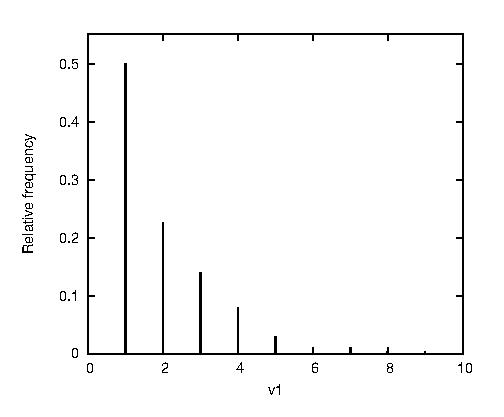
\includegraphics[width=0.5\textwidth]{hist_fr_v1.eps}}                
  \subfloat[Po přidání náhodných]{\label{fig:hist_fr_v2}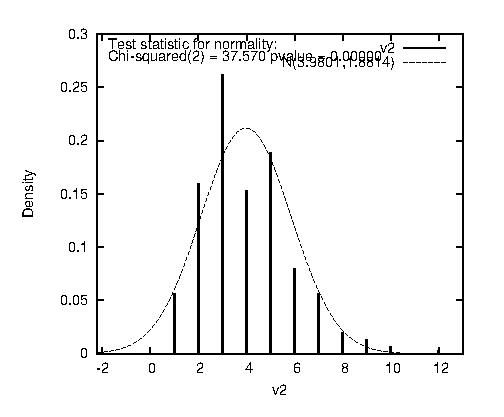
\includegraphics[width=0.5\textwidth]{hist_fr_v2.eps}}
  \caption{Histogram počtu přátelství}
  \label{fig:hist_fr}
\end{figure}
%\begin{center}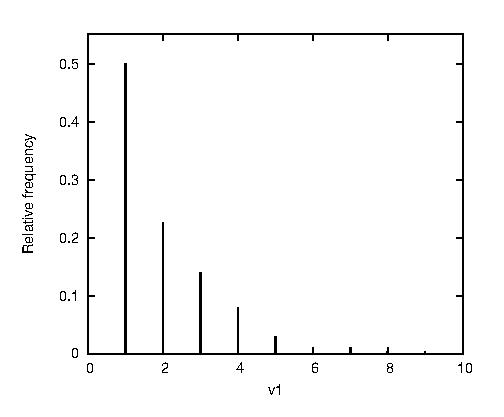
\includegraphics{hist_fr_v1.eps}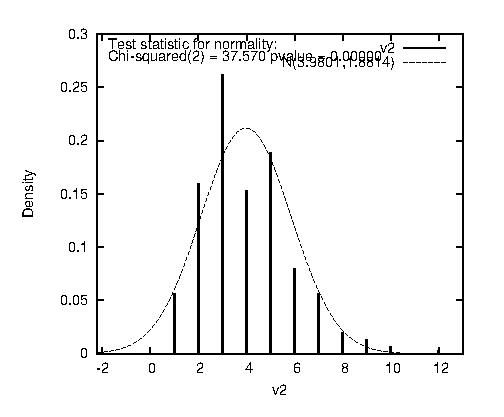
\includegraphics{hist_fr_v2.eps}\end{center}
\section{Prostředí}
Agenti jsou generování v izolovaném prostředí. Jsou přítomny tyto za běhu měnitelné konstanty:
\begin{description}
\item[\texttt{margin}] Marže pro prodejce z prodejní ceny. Nabývá reálných hodnot $(0,1)$.
\item[\texttt{monthly-fee}] Poplatek za členství placený v každém kole. Firma Oriflame jej nevybírá, je tedy určen spíše pro účely simulací.
\item[\texttt{manufacturing-cost}] Podíl výrobních nákladů na prodejní ceně produktů. Nabývá reálných hodnot $(0,1)$.
\end{description}
\section{Vlastnosti agenta \texttt{person}}
\label{sec:vl_agenta}
Agent \texttt{person} představuje v modelu jednoho člověka. Má tyto důležité vlastnosti:
\begin{description}
\item[\texttt{consupmtion}] Celé číslo udávající množství peněz, které daná osoba během jednom období může utratit za kosmetické výrobky, které je možno koupit v síti Oriflame. Je to část osobního rozpočtového omezení a považuje se za konstantní. Ve výchozím nastavení je generováno jako
$$\max\{100,\texttt{random-normal(1000,500)}\},$$
tj. náhodná hodnota z normálního rozdělení se střední hodnotou 1000, rozptylem 500, zdola omezená 100. Lidé s nižší spotřebou kosmetických výrobků ve skutečnosti samozřejmě existují, ale z pohledu této práce nejsou významní.
\item[\texttt{be-point}] Celé čislo znamenající bod ukončení činnosti. Za běhu se nemění. Členstvím v síti vznikají každému náklady. Tvoří je explicitní např. výdaje za cestu k zakazníkům a implicitní za čas obětovaný této práci. Obecně lze říci, že implicitní složka bude tím vyš\-ší, čím lépe na daný člověk placené hlavní zaměstnání. A tím se také zvyšuje jeho rozpočtové omezení. Proto existuje závislost mezi \texttt{consumption} a \texttt{be-point} vyjádřená
$$\max\{0.5\cdot\texttt{consumption},\texttt{consumption}\cdot\texttt{random-normal(1,0.5)}\},$$
což znamená minimálně polovina měsíční spotřeby, jinak násobek spotřeby se střední hodnotou 1 a rozptylem 0.5.
\item[\texttt{netmember?}] Příznak učující, zda je agent členem sítě -- prodejcem. Při inicializaci je nastaven na nepravdu a za běhu dojde k jeho změně, pokud se agent rozhodne vstoupit do prodejní sítě nebo z ní naopak vystoupit.
\end{description}
\section{Chování agenta \texttt{person}}
Chování vychází z jednoduché úvahy -- vyplatí se do sítě vstoupit a zůstat v ní? Lze jej tedy rozdělit na dvě části: podmínku vstupní a podmínku setrvání. Předpokládá se, že pokud se agent stane prodejcem, bude on a jeho přátelé svou potřebu kosmetických výrobků uspokojovat přednostně nákupem u něj. Ostatním agentům zboží neprodává.
\subsubsection{Vstupní podmínka}
Pokud je agentovi nabídnuto členství, přijme ho jestliže jeho očekávaný příjem převýší celkové ekonomické náklady. První část příjmů tvoří očekávaný výdělek z přímého prodeje, který lze přesně vypočítat, neboť agent zná spotřebu svou a svého bezprostředního okolí a tuto sumu pak jen vynásobí prodejní marží. Druhou částí je očekávaný příjem z budování skupiny prodejců, tj. přívádění dalších lidí k Oriflame. Jeho velikost může agent zpočátku pouze odhadnout, protože nevidí hloubějí do struktury sítě přátelství. Zde je určen podle vzorce, který přibližně odpovída výpočtu uváděnému skutečnými prodejci Oriflame. Příjmová strana je ještě vynásobena diferencí mezi současnou prodejní marží a tou, která byla platná při posledním odchodu agenta ze sítě. Pokud se v běhu simulace zvýší parametr \texttt{margin}, budou agenti reagovat zvýšením příjmových očekávání a naopak. Celkem je podmínka daná takto:
\[(\texttt{my-rev-exp} + \texttt{avg-srev-exp}) \cdot (1+\texttt{d-margin}) \geq \texttt{be-point} + \texttt{monthly-fee}\]
\begin{description}
\item[\texttt{my-rev-exp}] je očekávaný příjem z přímeho prodeje přátelům agenta. Pokud některému z nich může zboží dodávat více prodejců, je spotřeba rozdělena rovnoměrně mezi ně. Přesný postup je uveden v algortimu \ref{alg:myrevexp}.
\begin{algorithm}
\caption{Výpočet \texttt{my-rev-exp}}
\label{alg:myrevexp}
\begin{algorithmic}[]
\STATE \texttt{my-rev-exp} $\gets$ moje spotřeba $\cdot$ \texttt{margin}
\FORALL{$f\in$ moji přátelé}
  \STATE $n\gets 1 + $ počet přátel osoby $f$, kteří jsou prodejci
  \STATE $\texttt{my-rev-exp}\gets\texttt{my-rev-exp}+(\text{spořeba osoby }f \cdot \texttt{margin}) / n$
\ENDFOR
\end{algorithmic}
\end{algorithm}
\item[\texttt{avg-srev-exp}] je očekávaný příjem ze sponzoringu a skupin. Protože v rozhodování člověka je jistá setrvačnost, je dán jako průměr posledních deseti skutečných příjmů z této činnosti. Agent \texttt{person} má tedy 10 prvkovou frontu \texttt{exp-srev-list}, na jejíž konec se v každém kole přidá skutečný příjem ze skupin a vypadne poslední prvek. \texttt{avg-srev-exp} je pak roven průměru hodnot v této frontě. Při inicializaci je fronta naplněna hodnotami
\[ 0.09\cdot \text{suma spotřeby mých přátel}\cdot \text{počet mých přátel}^{1.3}.\]
To odpovídá odhadu uváděnému při nabídce členství v síti, tedy přítomnosti na 9\% úrovni a mocnině počtu přátel z důvodu větvění stromu.
\item[\texttt{d-margin}] je rozdíl mezi současnou \texttt{margin} a tou při posledním odchodu agenta ze sítě.
\end{description}
\subsubsection{Podmínka setrvání}
Vychází ze stejných úvah a je dána velmi podobně:
\[ \texttt{my-rev} + \texttt{avg-srev-exp} \geq \texttt{be-point} + \texttt{monthly-fee} \]
\texttt{my-rev} v tomto případě již není odhad, ale skutečná hodnota příjmu z přímeho prodeje. Tím jak se fronta \texttt{exp-srev-list} naplňuje skutečnými velikostmi výdělku ze skupin může dojít ke snížení jejího průměru a agentovi se pak vyplatí nebýt nadále prodejcem.
\section{Šíření prodejní sítě}
\label{sec:spread}
Na začátku je jeden agnet \texttt{person} určen jako zakladatel, je mu nastaveno \texttt{netmember?} na pravdu a \texttt{be-point} na 0, čímž je zajištěno, že nikdy nepřestane být prodejcem a prodejní síť se bude mít vždy odkud šířit. V každém kole je všem přátelům prodejců nabídnuto členství a dojde k vyhodnocení vstupní podmínky. Toto se děje nikoliv paralelně, ale postupně v náhodném pořadí, tj. pokud některé osobě mohou členství nabídnout dva nebo více prodejců, je zvolen jeden náhodný a ten si jej v případě splnění vstupní podmínky zařadí do svého podstromu grafu vztahů \texttt{sponsor}.

Je možne také zapnout volbu \texttt{random-join?}, která znamená, že v každém kole jeden náhodný agent nabídne členství jednomu náhodnému nečlenovi i mimo okruh svých přátel. To modeluje případ, kdy se prodejci snaží o nábor lidí např. na náměstích a u stánků v nákupních centrech.
 
Pokud není splněna podmínka setrvání, přestane agent být prodejcem a všechny jeho vztahy \texttt{sponsor} jsou převedeny na agenta ve stromu nad ním.
\section{Průběh kola a výpočty}
Nejprve se seznámíme s nejdůležitějšími body, pak se jim budeme věnovat podrobně. V každém kole probíhají tyto kroky:
\begin{enumerate}
\item Výpočet skutečného \texttt{my-rev} pro každého prodejce -- algoritmus \ref{alg:myrev}.
\item Výpočet výdělků ze skupin -- algoritmus \ref{alg:points} a funkce $SubnetRev$.
\item Vyhodnocení podmínky setrvání pro každého prodejce postupně v náhodném pořadí.
\item Vyhodnocení vstupní podmínky postupem popsaným v kapitole \ref{sec:spread}.
\item V případě zapnuté volby \texttt{random-join?} vyhodnocení vstupní podmínky pro náhodnou osobu.
\end{enumerate}
\begin{algorithm}
\caption{Výpočet skutečného \texttt{my-rev} pro každého prodejce}
\label{alg:myrev}
\begin{algorithmic}[]
\FORALL{$s\in$ prodejci}
  \STATE \texttt{my-rev }$s\gets$ spotřeba $s$ $\cdot$ \texttt{margin}
  \STATE\COMMENT{velmi podobně jako při výpočtu očekávání}
  \FORALL{$f\in$ přátelé $s$}
    \STATE $n\gets $ počet přátel osoby $f$, kteří jsou prodejci
    \STATE $\texttt{my-rev }s\gets\texttt{my-rev }s+(\text{spořeba osoby }f \cdot \texttt{margin}) / n$
  \ENDFOR
\ENDFOR

\end{algorithmic}
\end{algorithm}

\begin{algorithm}
\caption{Výpočet výdělků ze skupin}
\label{alg:points}
\begin{algorithmic}[]
\STATE {\bf function} $SubnetRev( p )$
\IF{$p$ nikoho nepřivedl}
  \STATE \texttt{srev-level} $p\gets$ podle \texttt{my-rev} $p$ odečti z tabulky \ref{tab:perc_level} procentní úroveň
  \STATE\COMMENT{nikoho nepřivedl, základ pro výdělek ze skupin tvoří pouze vlastní prodej}
  \STATE \texttt{my-srev} $p\gets\texttt{srev-level}\cdot\texttt{my-rev}$
  \STATE {\bf return} \texttt{my-rev}
\ELSE
  \STATE\COMMENT{spočítáme sumu spotřeby osoby $p$ a podstromu}
  \STATE $sum\gets\texttt{my-rev }p$
  \FORALL{$s\in$ osoby, které $p$ přivedl}
    \STATE $sum\gets sum + SubnetRev(s)$ \COMMENT{rekurzivní volání}
  \ENDFOR
  \STATE \texttt{srev-level} $p\gets$ podle $sum$ odečti z tabulky \ref{tab:perc_level} procentní úroveň
  \FORALL{$s\in$ osoby, které $p$ přivedl}
    \STATE $dperc\gets \texttt{srev-level } p - \texttt{srev-level } s$ \COMMENT{rozdíl procentních úrovní}
    \STATE \texttt{my-srev} $p\gets$ \texttt{my-srev} $p+dperc\cdot(\texttt{my-rev }s~/~\texttt{margin})$ \COMMENT{spotřeba podstormu vynásobená rozdílem procentních úrovní}
  \ENDFOR
  \STATE {\bf return} $sum$
\ENDIF 
\STATE {\bf end}
\\
\STATE spusť $SubnetRev($zakladatel$)$
\end{algorithmic}
\end{algorithm}
\clearpage
\section{Rozdíly modelu a skutečnosti}
Zde shrneme zjednodušení použitá při vytváření modelu:
\begin{itemize}
\item Tvorba sítě sociálních vztahů je nepostihuje v celé rozmanitosti, která je v reálné společnosti přítomna. Tato problematika může být předmětem zvláštního zkoumání.
\item Samotný rozsah sítě je z důvodu výpočetní kapacity omezen.
\item Chování agenta \texttt{person} je založeno ja jednoduché ekonomické úvaze. Skutečný člověk se rozhoduje mnohem komplexněji.
\item Model neuvažuje limit 100 bodů pro zisk výdělku ze skupin. To je odůvodněno tím, že člověk, který má možnost vysokého výdělku se jím nenechá odradit a vždy tuto podmínku nějakým způsobem splní, např. zvýšením své vlastní spotřeby kosmetických výrobků -- o tomto hovoří zkušenosti skutečných prodejců Oriflame. Zde však považujeme spotřebu za konstantní.
\end{itemize}
%
%
%
\chapter{Analýza výsledků simulací}
V této kapitole budeme provádět multiagentové simulace na modelu prodejní sítě Oriflame a analyzovat jejich výsledky. Pokud nebude uvedeno jinak pracujeme s výchozím modelem a základními parametry:\\[3mm]
$\texttt{number-of-persons}=\texttt{number-of-friendships}=300$ -- omezení z důvodu výpočetní kapacity\\
$\texttt{margin}=0.23$ -- marže vycházející z rovnice \ref{eq:pcnc}\\
$\texttt{monthly-fee}=100$ -- arbitrárně stanoveno\\
vlastnosti agenta \texttt{person} uvedené v sekci \ref{sec:vl_agenta}\\[3mm]
Data budou získána pomocí nástroje BehaviorSpace obsaženého v programu NetLogo. Ten umožňuje opakovaný běh modelu při různých parametrech, čímž lze získat rozsáhle a statisticky významné datové soubory.

K měření budou sloužit mimo jiné tyto veličiny:
\begin{description}
\item[\texttt{network-fee-revenue}] Příjem firmy z poplatků.
\item[\texttt{network-sale-revenue}] Příjem firmy z prodeje výrobků (za nákupní ceny).
\item[\texttt{revenue}] Součet předchozích dvou.
\item[\texttt{scost}] Náklady na výplatu sponzoringu a skupin.
\item[\texttt{mcost}] Výrobní náklady.
\item[\texttt{network-profit}] Celkový účetní zisk provozovatele sítě Oriflame bez fixních nákadů. 
\end{description}
Ke statistické analýze bude využit ekonometrický software GRETL\cite{gretl} verze 1.9.1 a tabulkový procesor Gnumeric\footnote{Gnumeric --- The Gnome Office Spreadsheet, \url{http://projects.gnome.org/gnumeric/}} 1.10.14.
\section{Šíření sítě}
Zde se budeme zkoumat šíření sítě a její výsledné vlastnosti. 
\subsection{Průběh šíření}
Bylo provedeno 100 nezavislých náhodných běhů pro výchozí parametry z úvodu kapitoly. Podmínkou ukončení je stabilizace sítě, tj. rovnost dvou po sobě následujících \texttt{network-profit}. Získaná data jsou v přiloženém souboru \texttt{spread1.csv}. Z nich odvozené popisné statistiky jsou v tabulce \ref{tab:spread1_desc}.
\begin{table}[h]
  \begin{center}
  \begin{tabular}{|r|r|r|r|}
  \hline
  Statistika&Počet členů na konci	&Maximum členů	&Počet kol do stabilizace\\\hline
  Průměr	&81.47	&217.2	&24.17\\
  Medián	&82	&218	&24\\
  Std. odchylka	&3.83	&6.67	&2.09\\
  Minimum	&72	&202	&20\\
  Maximum	&92	&234	&29\\\hline
  \end{tabular}
  \end{center}
  \caption{Popisné statistiky pro \texttt{spread1}}
  \label{tab:spread1_desc}
\end{table}
Vidíme, že průměrný běh trval 24 kol. Členy sítě se v průběhu stalo maximálně 217 osob z 300 a nakonec zůstalo 81, tedy přibližne čtvrtina. Časová řada počtu členů jednoho vybraného běhu je vidět na grafu \ref{fig:spread1_run}.
\begin{figure}[h]
  \centering
  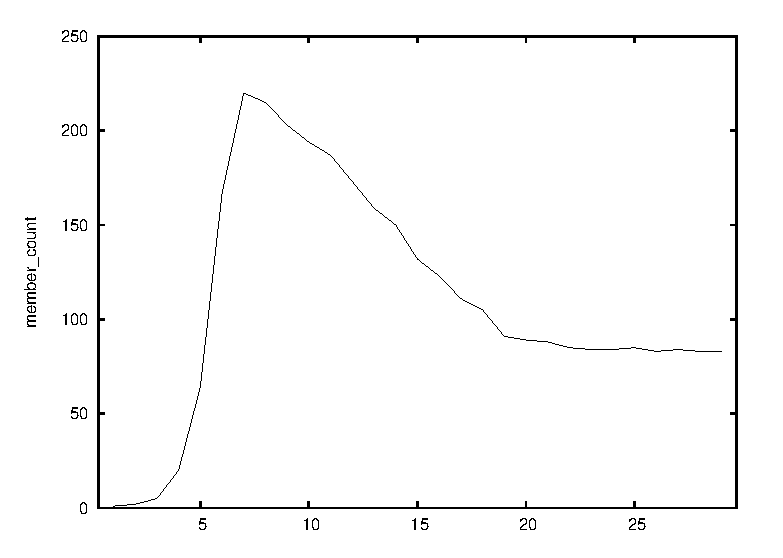
\includegraphics{member_count.eps}
  \caption{Vybraný běh simulace \texttt{spread1}}
  \label{fig:spread1_run}
\end{figure}
%\begin{center}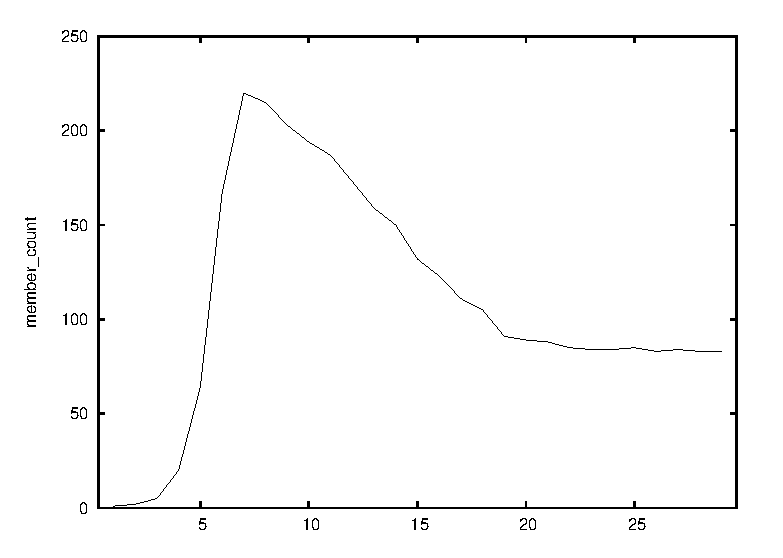
\includegraphics{member_count.eps}\end{center}
Je patrné, že síť se z počátku rychle rozrůstá díky velkým očekáváním. Ta ale nejsou většinou naplňena a dochází k postupnému úbytku.
\subsection{Vlastnosti agentů}
Nabízí se otázka, jakou vlastnost mají agenti, kteří v síti zůstali. Jedním důvodem může být nadprůměrný počet přátel. Za stejných podmínek jako v předchozím případě sestavíme simulaci. Výsledkem běhu je průměrný počet přátel pro člena sítě a pro všechny osoby. Data jsou k dispozici v souboru \texttt{spread2.csv}. Popisné statistiky jsou v tabulce \ref{tab:spread2_desc}.
\begin{table}[H]
  \begin{center}
  \begin{tabular}{|r|r|r|r|}
  \hline
  Statistika&Průměrný počet přátel pro člena	&Průměrný počet přátel pro všechny\\\hline
  Průměr	&5.44	&3.98\\

  Variance	&0.03	&0.00\\\hline
  \end{tabular}
  \end{center}
  \caption{Popisné statistiky \texttt{spread2}}
  \label{tab:spread2_desc}
\end{table}
\noindent
Hypotéza: $M_1=M_2$ proti $M_1>M_2$\\
P-hodnota testové statistiky $T = 9.51\cdot 10^{-97}$\\
Jednoznačně tedy zamítáme nulovou hypotézu a je zřejmé, že stálí členové sítě mají nadprůměrný počet přátel.\vspace{3mm}

Druhým důvodem může být malý \texttt{be-point}, což způsobí výhodnost členství. Simulaci provedeme stejným způsobem jako u počtu přátel. Statistiky vidíme v tabulce \ref{tab:spread3_desc}. Výsledky lze nalézt v souboru \texttt{spread3.csv}.
\begin{table}[H]
  \begin{center}
  \begin{tabular}{|r|r|r|r|}
  \hline
  Statistika&Průměrný \texttt{be-point} pro člena	&Průměrný \texttt{be-point} pro všechny\\\hline
  Průměr	&533.45	&1051.82\\

  Variance	&1279.18	&1896.18\\\hline
  \end{tabular}
  \end{center}
  \caption{Popisné statistiky \texttt{spread3}}
  \label{tab:spread3_desc}
\end{table}
\noindent
Hypotéza: $M_1=M_2$ proti $M_1>M_2$\\
P-hodnota testové statistiky $T = 3.06\cdot 10^{-109}$\\
Nade vší pochybnost opět zamítáme možnost rovnosti průměrů. Členové tedy maji obecně podprůměrný \texttt{be-point}.\vspace{3mm}

Z těchto dvou simulací je patrné, že prodejci se rekrutují z řad lidí s nižším příjmem a velkým počtem přátel. Model z tohoto pohledu věrně vystihuje realitu, neboť ve společnosti tuto skupinu tvoří převážně studenti a např. rodiče na mateřské dovolené -- největší část prodejců Oriflame.
\section{Vliv náborových akcí}
Jak již bylo uvedeno, někteří prodejci z vlastní iniciativy pořádají náborové akce, kde se snaží přivést k Oriflame i lidi mimo své přátele. Model to simuluje tak, že se v každém kole nabídne členství jednomu náhodnému nečlenovi. Budeme zjišťovat, zda-li to má význam pro počet členů po stabilizaci. Provedeme dvě simulace, první s \texttt{random-join?} vypnutým a druhý se zapnutým. V obou bude celkem 226 běhů modelu s \texttt{number-of-friendships} zvyšujícím se od 50 do 500 po krocích velikosti 2. Data jsou uložena v souborech \texttt{random-join1.csv} a \texttt{random-join2.csv}. Výsledné bodové grafy jsou na obrázku \ref{fig:random-join}. Metodou nejmenších čtverců byly nalezeny tyto regresní přímky:
\begin{figure}[h]
  \centering
  \subfloat[\texttt{random-join?} vypnuto]{\label{fig:random_join1}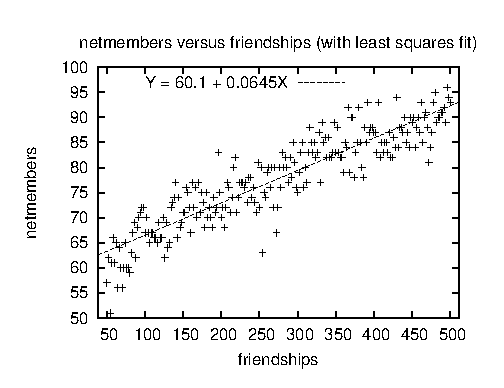
\includegraphics[width=0.5\textwidth]{random-join1-1.eps}}                
  \subfloat[\texttt{random-join?} zapnuto]{\label{fig:random_join2}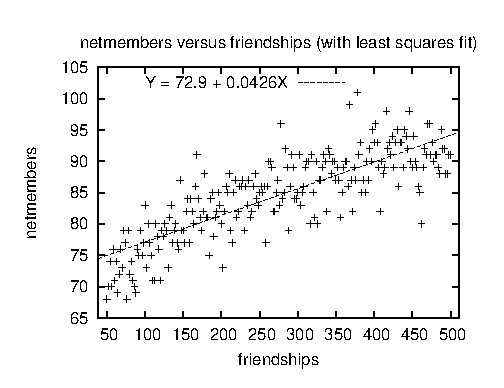
\includegraphics[width=0.5\textwidth]{random-join2-1.eps}}
  \caption{Bodový graf simulací \texttt{random-join} s OLS přímkou}
  \label{fig:random-join}
\end{figure}
\begin{itemize}
\item \texttt{random-join?} vypnuto\\
\begin{gather}
\widehat{\rm netmembers} = 
\underset{(0.61341)}{60.0865}
+\underset{(0.0020152)}{0.0644801}\,\mbox{friendships}
 \notag \\
T = 226 \quad \bar{R}^2 = 0.8197 \quad F(1,224) = 1023.8 \quad \hat{\sigma} = 3.9530 \notag
\end{gather}
\begin{center}

\begin{raggedright}
Test for normality of residual --\\
\quad Null hypothesis: error is normally distributed\\
\quad Test statistic: $\chi^2(2)$ = 2.93214\\
\quad with p-value = 0.230831\\
\vspace{1ex}
Breusch-Pagan test for heteroskedasticity --\\
\quad Null hypothesis: heteroskedasticity not present\\
\quad Test statistic: LM = 1.77929\\
\quad with p-value = $P$($\chi^2(1) >$ 1.77929) = 0.182237\\
\vspace{1ex}
\end{raggedright}

\end{center}

\item \texttt{random-join?} zapnuto\\
\begin{gather}
\widehat{\rm netmembers} = 
\underset{(0.62107)}{72.8508}
+\underset{(0.0020404)}{0.0426021}\,\mbox{friendships}
 \notag \\
T = 226 \quad \bar{R}^2 = 0.6591 \quad F(1,224) = 435.94 \quad \hat{\sigma} = 4.0024 \notag
\end{gather}
\begin{center}

\begin{raggedright}
Test for normality of residual --\\
\quad Null hypothesis: error is normally distributed\\
\quad Test statistic: $\chi^2(2)$ = 1.1743\\
\quad with p-value = 0.555909\\
\vspace{1ex}
Breusch-Pagan test for heteroskedasticity --\\
\quad Null hypothesis: heteroskedasticity not present\\
\quad Test statistic: LM = 0.0174692\\
\quad with p-value = $P$($\chi^2(1) >$ 0.0174692) = 0.894849\\
\vspace{1ex}
\end{raggedright}

\end{center}

\end{itemize}
V závorkách jsou uvedeny standardní chyby. Testy o normalitě reziduí a nepřítomnosti heteroskedasticity ve všech případech na 5\% hladině významnosti nulovou hypotézu nezamítají.

Z rovnic vidíme, že náborové akce jsou zvlášť výhodné pro skupiny lidí s nižšími počty přátel. Při $\texttt{number-of-friendships}=50$ a využití náborových akcí je počet prodejců o téměř 13 osob (20\%) vyšší než bez nich.
Existuje tam možnost vzniku slabých článků, které zabrání dalšímu šíření sítě. Koeficinet u friendships je naopak nižší. Tím dojde k průniku regresních přímek při $\texttt{number-of-friendships}=584$, což přibližne odpovídá průměrnému počtu přátel na osobu $5,84$. Pro prodejce z toho plyne doporučení, že pokud je počet přátelství v jejich okolí (za předpokladu jisté homogenity) vyšší než tato hodnota, není pro ně výhodné pořádat nábory, protože síť si ke všem najde cestu sama.
\section{Slabé články}
V předchozí části jsme zjistili existenci slabých článků, tj. agetů, přes které síť neprojde a její šíření se zastaví. Zde se je pokusíme identifikovat a objevit jejich společné vlastnosti. Slabý článek (bottleneck) bude určen tímto postupem:
\begin{enumerate}
\item Všem agentům se inicializujeme vlastnost \texttt{invited?} na nepravdu.
\item Necháme síť šířit standardním způsobem bez náhodných náborových akcí do stabilizace, příčemž všem agentům, kterým bylo nabídnuto členství nastavíme \texttt{invited?} na pravdu.
\item Projdeme všechny přátele všech agentů, kterým nebylo nabídnuto členství, a za slabý článek jsou označeni ti, kterým bylo nabídnuto členství.
\end{enumerate}
\begin{displaymath}
    \xymatrix{ A \ar[d] & \text{prodejce}  \\
               B \ar[d] & \text{slabý článek -- nikdy nepřijal členství} \\
               C & \text{nikdy nebylo nabídnuto členství} }
\end{displaymath}
\begin{center}
Šipka značí směr šíření sítě.
\end{center}
Zkoumejme nejprve, zda-li existuje závislost mezi \texttt{number-of-friendships} a počtem slabých článků. Sestavíme simulaci, který bude \texttt{number-of-friendships} v každém běhu v rozmezí 50 až 500 zvyšovat o 1. Data jsou uložena v souboru \texttt{bottleneck-count.csv}.
\begin{figure}[h]
  \centering
  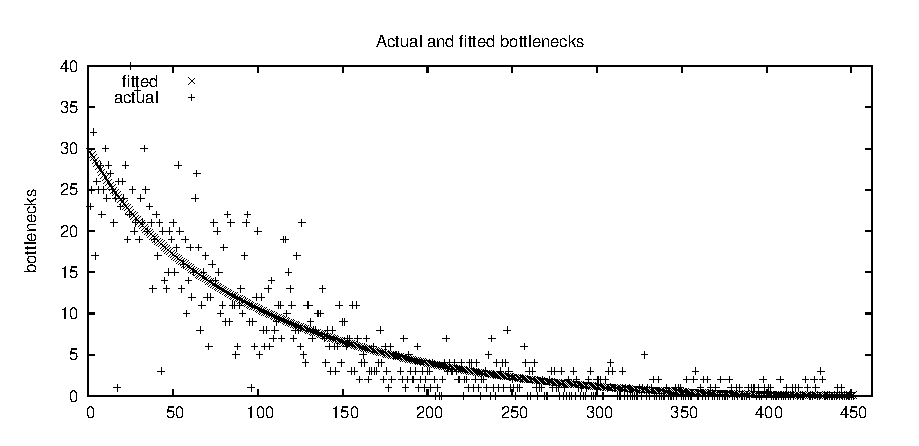
\includegraphics{bottleneck-count.eps}
  \caption{Běh simulace \texttt{bottleneck-count} s regresní křivkou}
  \label{fig:bottleneck-count}
\end{figure}
\begin{gather}
\widehat{\rm bottlenecks} = 
\underset{(6.2059)}{111.272}
-\underset{(1.3764)}{21.4307}\,\mbox{l\_friendships}
+\underset{(0.0052075)}{0.0440456}\,\mbox{friendships}
 \notag \\
T = 451 \quad \bar{R}^2 = 0.8278 \quad F(2,448) = 591.45 \quad \hat{\sigma} = 3.3252 \notag \\
\text{Vzhledem k přítomnosti heteroskedasticity byl použit estimátor HC1. } \notag \\
\text{\mbox{l\_friendships} značí přirozený logaritmus hodnot \mbox{friendships}.} \notag
\end{gather}
Vidíme, že s houstnocí sítí vcelku logicky dochází k rychlému poklesu počtu slabých čláků. Ideální hodnotou \texttt{number-of-friendships} pro další zkoumání se jeví 150, kdy již není počet slabých článků tak rozptýlen, ale stále je dost vysoký.

Provedeme simulaci se 100 běhy při $\texttt{number-of-friendships}=150$. Zkoumáme průměrný počet přátel a \texttt{be-point} pro všechny a pro slabé články. Výsledné hodnoty jsou v souboru \texttt{bottleneck1.csv}. Popisné statistiky obsahuje tabulka \ref{tab:bottleneck1_desc}. Z ní je patrné, že slabé články mají podprůměrný počet přátel a velmi nadprůměrný \texttt{be-point}. Doporučením pro prodejce v případě, že se s nekým takovým setkají, je pokusit se od něj získat alespoň kontakt na jeho známé a tím jej v síti přeskočit.
\begin{table}[h]
  \begin{center}
  \begin{tabular}{|r|r|r|r|r|}
  \hline
   & \multicolumn{2}{|c|}{Prům. počet přátel} & \multicolumn{2}{|c|}{Prům. \texttt{be-point}} \\\hline
	  &všichni	&slabé články	&všichni	&slabé články\\\hline
  Průměr	&3.00	&2.50	&1051.30	&1778.86\\
  Std. odchylka	&0.01	&0.23	&35.17	&260.47\\
  Minimum	&2.98	&2.00	&979.53	&867.00\\
  Maximum	&3.00	&4.00	&1142.78	&2440.33\\\hline
  \end{tabular}
  \end{center}
  \caption{Popisné statistiky \texttt{bottleneck1}}
  \label{tab:bottleneck1_desc}
\end{table}
\section{Optimální \texttt{margin} a \texttt{monthly-fee}}
Zde se budeme věnovat optimálnímu chování provozovatele prodejní sítě vzhledem k maximalizaci jeho zisku. Budeme předpokládat, že může stanovovat \texttt{margin} a \texttt{monthly-fee}, naopak podíl výrobních nákladů na prodejní ceně je v krátkém odbodí daný. Cílem bude nalézt funkci, která firmě v závislosti na jejích výrobních nákladech \texttt{manufacturing-cost} pomůže stanovit \texttt{margin} a \texttt{monthly-fee}. Zisk je stanoven jako rozdíl příjmových na nákladových veličin takto:
\[ \text{zisk}=\texttt{network-fee-revenue}+\texttt{network-sale-revenue}-\texttt{scost}-\texttt{mcost} \]
Přičemž platí funkční závislosti:
\begin{align}
\texttt{network-fee-revenue}=f_1(\texttt{fee},\texttt{margin})\notag\\
\texttt{network-sale-revenue}=f_2(\texttt{fee},\texttt{margin})\notag\\
\texttt{scost}=f_3(\texttt{fee},\texttt{margin})\notag\\
\texttt{mcost}=\frac{\texttt{network-sale-revenue}}{1-\texttt{margin}}\cdot\texttt{manufacturing-cost}\notag
\end{align}
Funkce $f_i$ zjistíme experimentálně. Budeme měnit \texttt{margin} v rozsahu $0.05$ až $0.9$ po kroku velikosti $0.01$ a \texttt{monthly-fee} na množině $\{0,50,100,150,200,250,300,350,400\}$. Pro každou iteraci provedeme 100 běhů modelu, celkem 77100 běhů. Pak z nich vypočítáme průměry jednotlivých veličin. Získaná data jsou přiloženém souboru \texttt{max-profit.csv}\footnote{Pozor, soubor má velikost 5.5MB, jeho otevření v tabulkovém procesoru je poměrně náročná operace.}. Ke zpracování průměrů byl vytvořen skript \texttt{max-profit.py} v jazyce Python\footnote{Python, \url{http://www.python.org/download/releases/3.2/}} a výsledek je uložen v souboru \texttt{max-profit-avg.tsv}. Na obrázku \ref{fig:max-profit-avg} vidíme bodové grafy funkcí $f$ pro $\texttt{monthly-fee}=100$ a zisku pro $\texttt{manufacturing-cost}=0.5$. 
\begin{figure}[h]
  \centering
  \subfloat[\texttt{network-fee-revenue}]{\label{fig:max-profit-avg-fr}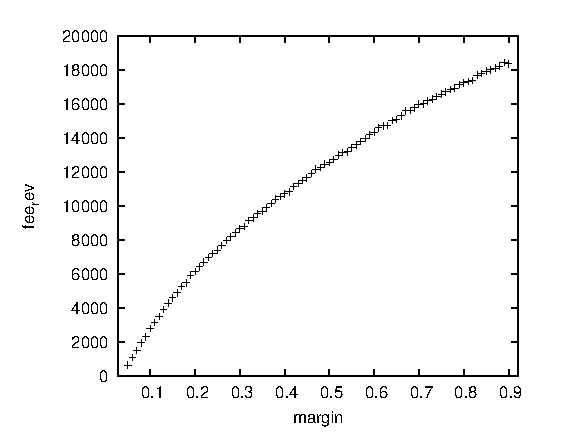
\includegraphics[width=0.5\textwidth]{max-profit-avg-fr.eps}}                
  \subfloat[\texttt{network-sale-revenue}]{\label{fig:max-profit-avg-sr}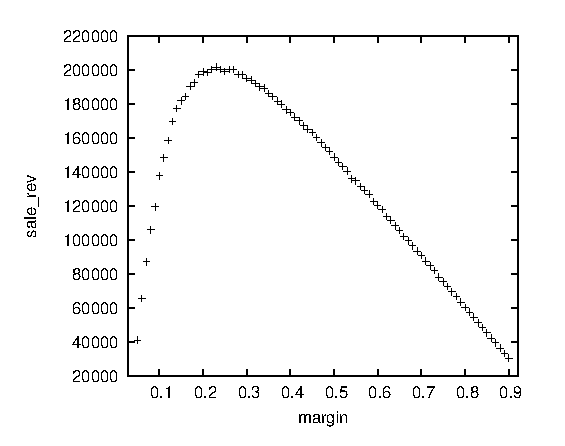
\includegraphics[width=0.5\textwidth]{max-profit-avg-sr.eps}}\\
  \subfloat[\texttt{scost}]{\label{fig:max-profit-avg-sc}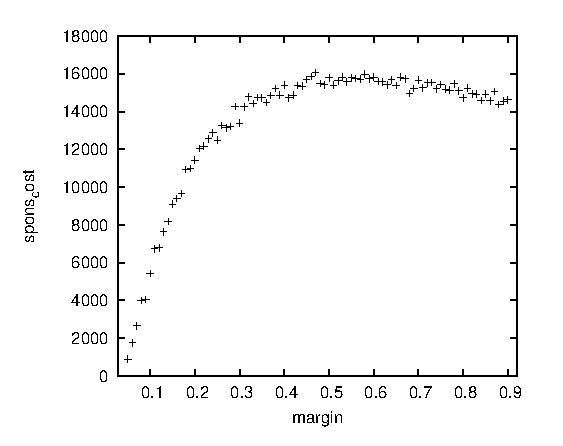
\includegraphics[width=0.5\textwidth]{max-profit-avg-sc.eps}}                
  \subfloat[zisk pro $\texttt{manufacturing-cost}=0.5$]{\label{fig:max-profit-avg-profit05}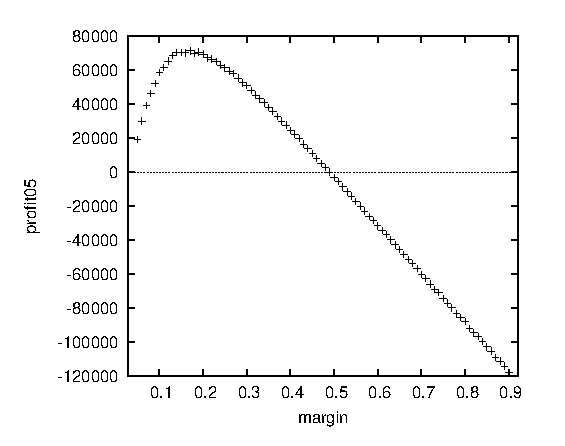
\includegraphics[width=0.5\textwidth]{max-profit-avg-profit05.eps}}\\
  \caption{Bodové grafy \texttt{max-profit-avg} pro $\texttt{monthly-fee}=100$}
  \label{fig:max-profit-avg}
\end{figure}
Tabulka \ref{tab:max-profit2} je hledanou pomůckou pro stanovení optimálních \texttt{margin} a \texttt{monthly-fee} podle \texttt{manufacturing-cost}. Např. pro $\texttt{manufacturing-cost}=0.4$ je predikován maximální zisk při $\texttt{margin}=0.18$ a $\texttt{monthly-fee}=50$. Nicméně zisk pro $\texttt{monthly-fee}=0$ je pouze o 92 jednotek nižší, což by firmě jistě nepokrylo administrativní náklady spojené s jeho výběrem, a je tak lepší jej zrušit a stanovit $\texttt{margin}=0.16$.
\begin{table}[h]
\begin{center}
\begin{tabular}{|l|r|r|r|r|r|r|r|}
\hline
fee & \multicolumn{1}{l|}{mc 0.1} & \multicolumn{1}{l|}{mc 0.2} & \multicolumn{1}{l|}{mc 0.3} & \multicolumn{1}{l|}{mc 0.4} & \multicolumn{1}{l|}{mc 0.5} & \multicolumn{1}{l|}{mc 0.6} & \multicolumn{1}{l|}{mc 0.7} \\ \hline
0 & 0.19 & 0.19 & 0.16 & 0.16 & 0.14 & 0.12 & 0.11 \\ 
 & 169666 & 144109 & 118721 & 94848 & 71341 & 49294 & 29318 \\ \hline
50 & 0.22 & 0.19 & 0.18 & 0.18 & 0.15 & 0.14 & 0.11 \\ 
 & 170435 & 144191 & 119404 & 94950 & 71435 & 49328 & 29609 \\ \hline
100 & 0.23 & 0.2 & 0.19 & 0.19 & 0.17 & 0.14 & 0.13 \\ 
 & 169886 & 143896 & 119212 & 94845 & 71374 & 49700 & 29440 \\ \hline
150 & 0.22 & 0.22 & 0.22 & 0.2 & 0.17 & 0.17 & 0.13 \\ 
 & 168971 & 143790 & 118608 & 94225 & 71077 & 48896 & 29131 \\ \hline
200 & 0.26 & 0.23 & 0.23 & 0.19 & 0.19 & 0.17 & 0.14 \\ 
 & 168857 & 142715 & 117718 & 93675 & 70882 & 48485 & 28298 \\ \hline
250 & 0.25 & 0.25 & 0.22 & 0.22 & 0.19 & 0.18 & 0.14 \\ 
 & 167459 & 142190 & 117126 & 93269 & 69527 & 48065 & 27933 \\ \hline
300 & 0.29 & 0.27 & 0.24 & 0.22 & 0.22 & 0.19 & 0.16 \\ 
 & 166961 & 141178 & 115795 & 91791 & 68810 & 47289 & 27183 \\ \hline
350 & 0.29 & 0.29 & 0.29 & 0.23 & 0.23 & 0.19 & 0.18 \\ 
 & 166893 & 140992 & 115092 & 91208 & 68273 & 46403 & 27071 \\ \hline
400 & 0.3 & 0.28 & 0.28 & 0.24 & 0.24 & 0.21 & 0.18 \\ 
 & 165112 & 139664 & 114750 & 90501 & 67643 & 46177 & 27058 \\ \hline
\end{tabular}
\end{center}
\caption{Optimální \texttt{margin} a z nich vypočítaný zisk pro dané \texttt{manufacturing-cost} a různé \texttt{monthly-fee}}
\label{tab:max-profit2}
\end{table}
Na obrázku \ref{fig:max-profit-04-f0} vidíme bodový graf zisku v závisloti na \texttt{margin} pro $\texttt{monthly-fee}=0$ a $\mbox{\texttt{manufacturing-cost}=0.4}$. Firmou Oriflame stanovený $\texttt{margin}=0.23$ je těsně na hranici, kde už začíná zisk rychle klesat. Predikovaný zisk je přibližne o 10\% nižší než maximum. Firma však takto může tvrdit, že prodejce bude mít výdělek 30\% (byť z nákupních cen). To je zřejmě pro mnohé pychologická hranice, což tento model do vstupní podmínky nezahrnuje.
\begin{figure}[h]
  \centering
  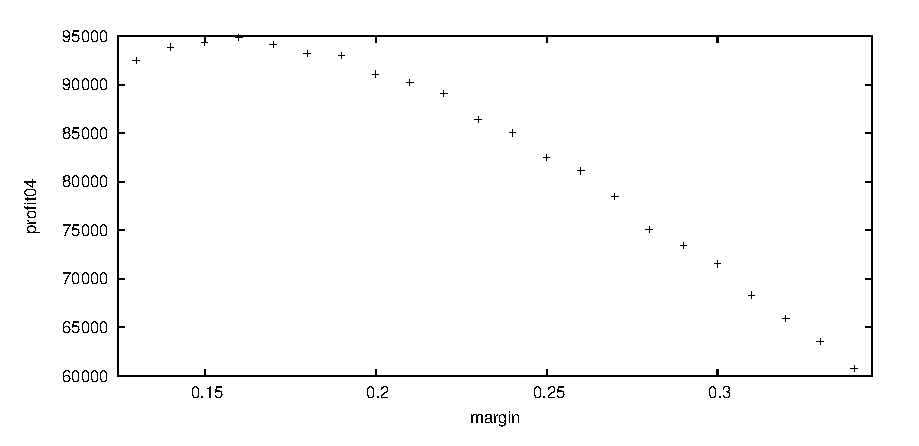
\includegraphics{max-profit-04-f0.eps}
  \caption{Zisk pro $\texttt{monthly-fee}=0$ a $\texttt{manufacturing-cost}=0.4$}
  \label{fig:max-profit-04-f0}
\end{figure}

Nyní se na tabulku \ref{tab:max-profit2} podívejme z toho pohledu, že firma z psychologických a marketingových důvodů chce stanovit $\texttt{margin}=0.23$. Pak odvodíme, že pro \mbox{$\texttt{manufacturing-cost}=0.4$} je nejziskovější vybírat $\texttt{monthly-fee}=350$. Jak bylo uvedeno v kapitole 1, existuje hranice 100 BO (což odpovídá přibližne 1380 Kč obchodního obratu) pro výplatu výdělku ze sponzorování. Toto a další faktory jako rozsáhlost katalogu, snadnost nákupu atd. vedou prodejce ke zvýšení spotřeby kosmetických výrobku prokázanému zkušeností, což model nezahrnuje z důvodu složité kvantifikovatelnosti. Tento jev lze však vnímat jako jistý skrytý poplatek. Zda dodatečný zisk ze zvýšené spotřeby dosahuje měsíční výše 350 zde není možné určit. Tato otázka může být předmětem dalšího zkoumání.

\chapter*{Závěr}
\addcontentsline{toc}{chapter}{Závěr}
\addtocounter{chapter}{1}
\begin{thebibliography}{9}

\bibitem{gretl}
COTTRELL, Allin; LUCCHETTI, Riccardo. Gnu Regression, Econometrics and Time-series Library [online]. Květen 2011 [cit. 2011-05-20].  Gretl User’s Guide. Dostupné z WWW: \url{http://sourceforge.net/projects/gretl/files/manual/}
\bibitem{epstein}
EPSTEIN, Joshua M.; AXTELL, Robert. Growing artificial societies : social science from the bottom up. Cambridge, Mass. : MIT Press,  1996. 208 s. ISBN 0262550253.
\bibitem{gilbert}
GILBERT, G. Nigel. Agent-based models. Los Angeles : Sage Publications,  c2008. xiii, 98 s. ISBN 9781412949644.
\bibitem{koop}
KOOP, Gary. Introduction to econometrics. Chichester : John Wiley \& Sons,  2008. 371 s. ISBN 9780470032701.
\bibitem{mankiw}
MANKIW, N. Gregory; SOJKA, Milan. Zásady ekonomie. 1. vyd. Praha : Grada,  1999. 763 s. ISBN 8071698911.
\bibitem{oriflame}
 Manuál kosmetického poradce Oriflame. Interní dokument. Aktualizace prosinec 2009. [s.l.] : [s.n.],  [2009]. 31 s. Katalogové číslo Oriflame 91571.
\bibitem{netlogo}
 NetLogo Home Page [online]. 2011-04-03 [cit. 2011-05-20].  NetLogo User Manual. Dostupné z WWW: \url{http://ccl.northwestern.edu/netlogo/docs/}
\end{thebibliography}
\chapter*{Uživatelská příručka}
\addcontentsline{toc}{chapter}{Uživatelská příručka}
\addtocounter{chapter}{1}
\subsubsection{velky model}
\subsubsection{???zjednoduseny model}
bez sponzorovani - je tam lepe videt neprima umera mezi ziskem firmy a vysi margin+fee
\end{document}

